%\documentclass[10pt,a4paper]{article}
\documentclass[nojss]{jss}

\usepackage[utf8]{inputenc}
%%\usepackage[final]{pdfpages} %% for including pdf appendix

%\usepackage{a4wide}
%\setlength{\parskip}{0.5ex plus0.1ex minus0.1ex}
%\setlength{\parindent}{0em}

%\usepackage[round,longnamesfirst]{natbib}
%\usepackage{hyperref}

%%% for tabulars
\usepackage{rotating}
\usepackage{multirow}

%%% for hanging paragraph
\usepackage{hanging}

%\newcommand{\strong}[1]{{\normalfont\fontseries{b}\selectfont #1}}
\newcommand{\class}[1]{\mbox{\textsf{#1}}}
\newcommand{\func}[1]{\mbox{\texttt{#1()}}}
%\newcommand{\code}[1]{\mbox{\texttt{#1}}}
%\newcommand{\pkg}[1]{\strong{#1}}
\newcommand{\samp}[1]{`\mbox{\texttt{#1}}'}
%\newcommand{\proglang}[1]{\textsf{#1}}
\newcommand{\set}[1]{\mathcal{#1}}

\linespread{1.6}

%\usepackage{Sweave}

\author{John Forrest\\Southern Methodist University \And
    Michael Hahsler\\Southern Methodist University}
\title{stream: A Framework for Data Stream Modelling in R}

\Plainauthor{John Forrest, Michael Hahsler}
\Plaintitle{Introduction to stream --
    A framework for modelling data streams and performing common
    data mining tasks}
\Shorttitle{Introduction to stream}

%% an abstract and keywords
\Abstract{
In recent years, data streams have become an increasingly important area of research. Common data mining tasks associated with data streams include classification and clustering. Due to both the size and the dynamic nature of data streams, it is often difficult to obtain real-time stream data without the overhead of setting up an infrastructure that will generate data. Our framework is designed to remove the overhead of building an infrastructure for generating data streams when performing research in data stream mining. We have built the framework in \proglang{R}, a popular tool for data mining and statistical analysis with the intent that researchers will be able to easily integrate our framework into their existing work. In this paper we introduce the implementation of \pkg{stream}, an \proglang{R} package that provides an intuitive interface for experimenting on data streams and their applications. \pkg{stream} is a general purpose tool that can model data streams and perform data mining tasks on the generated data. It has the ability to replay the requested data for other data mining tasks if needed, or read data streams from other sources and incorporate them into the framework.
}
\Keywords{data stream, data mining, cluster, classification}
\Plainkeywords{data stream, data mining, cluster, classification} %% without formatting


\Address{
	Michael Hahsler\\
	Computer Science and Engineering\\
	Lyle School of Engineering\\
	Southern Methodist University\\
	P.O. Box 750122 \\
	Dallas, TX 75275-0122\\
	E-mail: \email{mhahsler@lyle.smu.edu}\\
	URL: \url{http://lyle.smu.edu/~mhahsler}
}

\begin{document}
%\maketitle

\clearpage
\tableofcontents
\clearpage

\section{Introduction}

In recent years, data streams have become an increasingly important area of research. Common data mining tasks associated with data streams include classification and clustering \citep{stream:Aggarwal:2009}. Data streams are defined as ordered sequences of continually arriving points. The characteristic of continually arriving points introduces an important property of data streams is also their greatest challenge: their potentially infinite size. Due to the dynamic size of data streams, a significant amount of research involving data streams is spent on how to accurately summarize the data in real time so that it can be used in traditional data mining algorithms. Most data mining tasks for data streams are composed of two components: an online component which summarizes the data, and an offline component which uses these summaries as input to traditional algorithms to generate a prediction or clustering from the data.


The majority of the available data stream processing algorithms adhere to these properties:

\begin{itemize}
	\item \textbf{Single pass:} The incoming instances are processed no more than a single time
	\item \textbf{Finite:} The stored data will use a finite amount of space and time
	\item \textbf{Real-time:} A prediction can be generated upon request from the current snapshot of the stream
\end{itemize}


The names for these properties vary depending on the algorithm, but the core definitions remain the same across all data stream processing techniques. Another common property found in many techniques is the inclusion of a temporal structure due to the concept drift found in many streams \citep{stream:Masud+Chen+Khan+Aggarwal+Gao+Han+Thuraisingham:2010}.


Common data streams include text streams like Twitter activity, the Facebook news-stream, Internet packet data, stock market activity, output from sensor arrays, etc. The volume of data and its applications will only continue to increase as more techniques are developed to automatically record our day-to-day interactions with technology (credit card transactions, Internet and phone usage) to databases for use in behavioral mining \citep{stream:Aggarwal:2007}. Our goal with \pkg{stream} is provide a framework for experimentation that can generate data streams with specific properties based on the needs of the experiment. We aim to reduce the overhead that researchers spend on the creation of an experimental stream infrastructure so that they may focus more on innovative algorithms that can be used to mine real-world data streams.


When developing a new technique for any application, a vital step in the development process is the evaluation against existing methods in the field. Although an important step, the evaluation of a stream processing algorithm is often overlooked because of the challenging setup. Not only is it difficult to obtain implementations of leading algorithms to benchmark against, there are many other variables that often change between implementations: the programming language, development environment, expected input and output, etc. Additionally, the same data needs to be used for each experiment in order to accurately benchmark the performance against one another; and more importantly, the size of the data used in data stream processes cannot be trivial because the way the algorithms handle very large streams is a key feature. Both of these tasks make it a formidable challenge to accurately benchmark any new stream processing technique against existing algorithms.


The two most well-known tools for the benchmarking of traditional data mining methods are WEKA and \proglang{R} \citep{stream:Hall+Frank+Holmes+Pfahringer+Reutemann+Witten:2009, stream:R:2005}. The WEKA Data Mining Sofware is developed and maintained by the Machine Learning Group at the University of Waikato and consists of an interactive graphical user interface for low entry users. It is built in \proglang{Java} and supports easy integration of new techniques through its plug-in interface. At the other end of the spectrum is \proglang{R}, an environment for data mining and statistical computing that is operated solely by writing code from the command line interface or the input of script files. It supports extension in several forms: through \proglang{R} packages (software applications written in the \proglang{R} programming language), \proglang{Java}, and \proglang{C}/\proglang{C++}. In fact, since \proglang{R} allows extensibility by \proglang{Java}, there is a WEKA package available in \proglang{R} that uses the \proglang{Java} code from the standalone WEKA implementation.


To solve the problem of benchmarking data stream processes in \proglang{Java}, another team at the University of Waikato has developed Massive Online Analysis (MOA), a framework that has been built in WEKA's image \citep{stream:Bifet+Holmes+Kirkby+Pfahringer:2010}. MOA has a variety of tools that allows researchers to generate streams, perform data stream classification, and to perform data stream clustering. However, MOA only fills in one end of the spectrum, and to correspond to the other side, we have developed \pkg{stream}, an \proglang{R} package that performs many of the required tasks in the \proglang{R} environment but also allows the extensibility of data mining techniques in ways that MOA can't; namely development in \proglang{R} and \proglang{C}/\proglang{C++}. Additionally, \pkg{stream} will be compataible with \textit{REvolution R}, a commercial version of \proglang{R} that is optimizied for server environments that deal with terabytes of data. This will allow users that have access to \textit{REvolution R} to push the performance comparison of data stream applications that isn't possible in the open source version of \proglang{R} \citep{stream:revolutionR:2010}.


In this paper we discuss the design of \pkg{stream}, and how it can be used to compare data stream processing techniques. In our current implementation of \pkg{stream}, we have developed two main components: a component for generating stream data, and a component for performing data stream tasks, generally either clustering or classification, using the generated data. Each of these components is accompanied by examples demonstrating the capabilities of the framework. 


The paper is organized as follows. We first introduce the goal of \pkg{stream}, and our motivation in creating an experimental framework for modeling data streams. Following the introduction, we then provide background information on data streams, as well as common data mining tasks: clustering and classification. This is an important section if you are unfamiliar in this area of research. Resources are also given that offer further information on each area. This section is followed by the design of the \pkg{stream} package in Section~\ref{sec:design}. The design section covers the design of each component, how they interact with one another, and how to extend the components as a developer. Section~\ref{sec:examples} consists of examples in \proglang{R} that show the generation of data streams, data mining tasks performed on the streams created, and explanations that detail the resulting objects. Section~\ref{sec:conclusion} outlines our future plans for the framework and concludes the paper.

\section{Background}
\label{sec:background}

Due to advances in data gathering techniques, it is often the case that data is no longer viewed as a static collection, but rather as a dynamic set, or stream, of incoming data points. Nearly all of our interactions with technology are generating these data points which, in conjunction with other users’ interactions, can be seen as a very large data stream. As mentioned in the introduction, the volume and the infinite nature of these data streams provide challenging properties: single-pass, finite, and real-time. A thorough introduction to data streams can be found in \cite{stream:Aggarwal:2007} . The most common data stream mining tasks are clustering and classification. The rest of this section will give background information in these two areas, followed by the introduction of the MOA Framework—a framework that provides tools to perform both of these tasks on modeled data streams. The current version of \pkg{stream} only contains implementation for data stream clustering, so the classification section will provide a briefer overview.

\subsection{Data Stream Clustering}
\label{sec:background:dsc}

Traditional cluster analysis is an unsupervised data mining technique, meaning that there is no user intervention on the algorithms that group data points into meaningful classes (clusters) based upon certain attributes. Ideally, the data points that are clustered into a single class will be similar to one another, and dissimilar to data points in other classes. Unlike classification, which will be introduced in the next section, there is no pre-determined meaning of the classes, and it is up for the user to decide what the generated clusters mean. Most traditional clustering methods are multi-pass, meaning that they examine the input data set multiple times before generating the final result. For more detail on clustering outside of data streams, \citep{stream:Dunham:2002} and \citep{stream:Tan+Steinbach+Kumar:2006} each have chapters dedicated to cluster analysis and popular algorithms.


The data stream properties outlined previously render traditional clustering techniques unusable in their current form. New techniques were introduced to transform the data stream so that it can be used by the original clustering techniques. In general, data stream clustering algorithms consist of an online-offline architecture. The online component refers to the new data stream aspect of the algorithm that summarizes the data points into micro-clusters so that they can be used in the offline component. The offline part of these algorithms is executed upon the user’s command (the real-time property) and uses the centers of the micro-clusters as input data into clustering algorithms, such as \textit{k-means} or \textit{DBSCAN}. 


The accurate, yet efficient generation of micro-clusters is the goal behind the online component of data stream clustering algorithms. The offline component consists of algorithms that have been around for many years and their performance is well defined. Thus, the focus of new techniques in data stream clustering focus on how to summarize the incoming data effectively. Summarizing the incoming data points into micro-clusters ensures that the input to the offline component is constrained to a finite space. Recent algorithms such as \citep{stream:Cao+Ester+Qian+Zhou:2006} and \citep{stream:Wan+Ng+Dang+Yu+Zhang:2009} use a density-based approach to calculate micro-clusters, but there are a variety of different techniques used in \citep{stream:Guha+Meyerson+Mishra+Motwani+O'Callaghan:2003, stream:Aggarwal:2009, stream:Hahsler+Dunham:2010c, stream:Aggarwal+Han+Wang+Yu:2003}. 


To maintain a finite number of micro-clusters, a pruning function is often associated within the summarization process that discards micro-clusters that have become outliers. Outliers can be determined by data points that don’t have enough related instances to constitute a micro-cluster, or micro-clusters that have become stale—no new data points have been added to them recently. The latter case occurs when the structure of the data stream changes as a function of time.


In \pkg{stream}, our goal with data stream clustering is to separate the online component from each data stream clustering algorithm and use it as its own entity. We can then compare the performance of the online components of each algorithm when paired with a selected offline component. This is a feature unique to the \pkg{stream} framework. We focus on the online component of the algorithms because \proglang{R} already contains definitions for many of the offline components used, and the novelty of many of the algorithms is in the online component. Section~\ref{sec:design} discusses what data stream clustering algorithms are currently available in the framework, and how they can be operated upon.

\subsection{Data Stream Classification}
\label{sec:background:dscl}

Although there is no support of data stream classification in the current form of \pkg{stream}, it is one of the most popular data mining tasks and can easily be added due to the extensibility of \pkg{stream}. 


Classification is another data mining technique that groups related data into groups, or classes. Classification is known as a supervised learning technique because of the training phase in which the input data consists of a data set and the corresponding classes of its data points. The classification technique then examines the input and generates a model from the data. The model is then used to assign classes to new data according to what was learned during the training phase. \citep{stream:Dunham:2002} and \citep{stream:Tan+Steinbach+Kumar:2006} again provide detailed chapters on traditional classification and its applications.

\subsection{The MOA Framework}
\label{sec:background:moa}

MOA is a framework for both stream classification and stream clustering \citep{stream:Bifet+Holmes+Kirkby+Pfahringer:2010}. It is the first experimental framework to provide easy access to multiple algorithms, as well as tools to generate data streams to use to measure the performance of the algorithms. 


The workflow in MOA consists of three main steps: 1) the selection of the data stream model (referred as data feeds or data generators); 2) the selection of the algorithm in which the generated data will be used; and 3) the evaluation of the performance. After each step is complete, a report is generated that contains the performance evaluation as well as the results from the data mining task performed. The evaluation step and results from the experiments run differ based on the task—classification results are shown as a text file, while clustering results have a visualization component that charts both the micro-clusters calculated and the change in performance metrics over time.


The MOA framework is an important pioneer in experimental data stream frameworks. Many of the clustering techniques available in stream are from the MOA framework.

\section{The \pkg{stream} Framework}
\label{sec:design}

There are two main components to the \pkg{stream} framework which we built them with the intent of being 'base classes' from which all other classes in the framework will extend from. Figure~\ref{figure:workflow}  shows a high level view of the interaction of the components. The two components correspond to the steps taken in every learning algorithm: DataStreamData (DSD) refers to selecting or generating the data while DataStreamTask (DST) refers to selecting the data stream process that will use the input data. The figure demonstrates the simplicity of the framework. We start by creating a DSD, then feed the data generated by the DSD into a DST object, and finally we can obtain the results from the DST object. DSTs can be any type of data streaming mining task, most commonly classification or clustering algorithms. This section will outline the design principles introduced in \pkg{stream}, and the following subsections will cover the design of each of the components. 

\begin{figure}
\centering
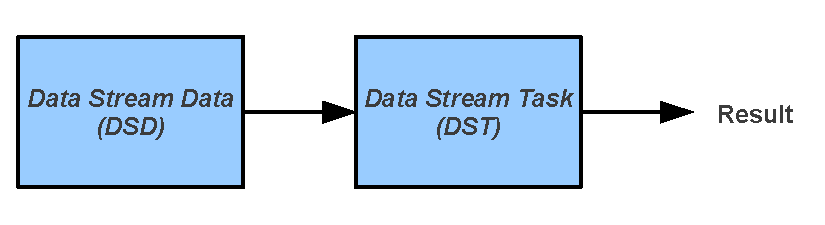
\includegraphics{architecture}
\caption{A high level view of the \pkg{stream} architecture.}
\label{figure:workflow}
\end{figure}

Each of these components has been abstracted into a lightweight interface that can be extended in either \proglang{R}, \proglang{Java}, or \proglang{C}/\proglang{C++}. Our current implementation contains both components that have been developed solely in \proglang{R}, and others that use an \proglang{R} wrapper for the underlying \proglang{Java} implementation from the MOA framework. The subsections following will go into more detail about the individual components followed by how they interact with one another.


All of the experiments must be run either directly in the \proglang{R} environment from the command line or as .R script files that can be piped into \proglang{R}. Currently there is no support in scaling the resources used by \pkg{stream} to simulate a different computing environment (i.e., a hand-held device versus a server), similar to how the MOA framework operates. However, the software experiments will scale with the computer hardware of the system \proglang{R} is being run on. As mentioned before, \pkg{stream} will also work on \textit{REvolution R}, an optimized commercial version of \proglang{R} that is designed to work on server architectures composed of multi-cores and can deal with terabytes of data at a time \citep{stream:revolutionR:2010}.


The \pkg{stream} package uses the S3 class system in \proglang{R}. The package has been validated by the command \code{R CMD check} which runs a series of 19 checks that covers all aspects of the package. Because there is no direct support for object oriented concepts in \proglang{R}, we have built the architecture in a specific way to emulate important principles such as data abstraction, modularity, encapsulation, and polymorphism. The first two concepts are trivial in their implementation in that we simply designed the class hierarchy so that the main components of the framework are loosely coupled and the underlying implementation details of each of them (whether they are in \proglang{R}, \proglang{Java}, or \proglang{C}/\proglang{C++}) are abstracted behind a standard \proglang{R} interface. Encapsulation principles are maintained by incorporating an immutable \proglang{R} list with each class. A \code{list} in \proglang{R} is an associative map that associates a variable name to a corresponding object. The \code{list} members that are exposed are similar to public members in a high level programming language.


Polymorphism is achieved by associating a 'class', or set of classes to the specific objects that are created. For example, the DataStreamClusterer (DSC) class of \code{DSC_tNN} (for the threshold nearest neighbor clustering algorithm) can be identified by any of these three classes: \code{DSC}, the base class of all DSCs; \code{DSC_R}, because it is implemented directly in \proglang{R}; or \code{DSC_tNN}, its specific class. This allows models the concept of polymorphism in that the user simply has to call a generic function, such as \code{get_points()}, and the appropriate function call will be executed based on the classes the DSC object inherits. 

\subsection{DataStreamData}
\label{sec:design:dsd}

The first step in the \pkg{stream} workflow is to select a DSD generator. Figure~\ref{figure:dsd} shows the UML relationship of the DSD classes \citep{stream:Fowler:2003}. All DSD classes extend from the abstract base class, \code{DataStreamData}. The current available classes are \code{DSD_Gaussian_Static}, a DSD that generates static cluster data with a random gaussian distribution; \code{DSD_Gaussian_Dynamic}, a class similar to the previous one except with dynamic data; \code{DSD_MOA}, a data generator from the MOA framework with an \proglang{R} wrapper; \code{DSD_ReadStream}, a class designed to read data from \proglang{R} connections; and finally, \code{DSD_DataFrame}, a DSD class that wraps local \proglang{R} data as a data stream. Additional DSD classes will also extend from the base class, as denoted by the ellipsis in the diagram.


The most common input parameters for the creation of DSD classes are \code{k} number of clusters, and \code{d} number of dimensions. We use the term cluster loosely here in that it refers to where data points will be generated from rather than a calculated cluster from an algorithm. Often associated with \code{k} and \code{d} are means and standard deviations for each dimension of each cluster (where \code{mu} denotes the matrix of means and \code{sigma} denotes the covariance matrix), and a probability vector that weighs the importance of the defined clusters.

\begin{figure}
\centering
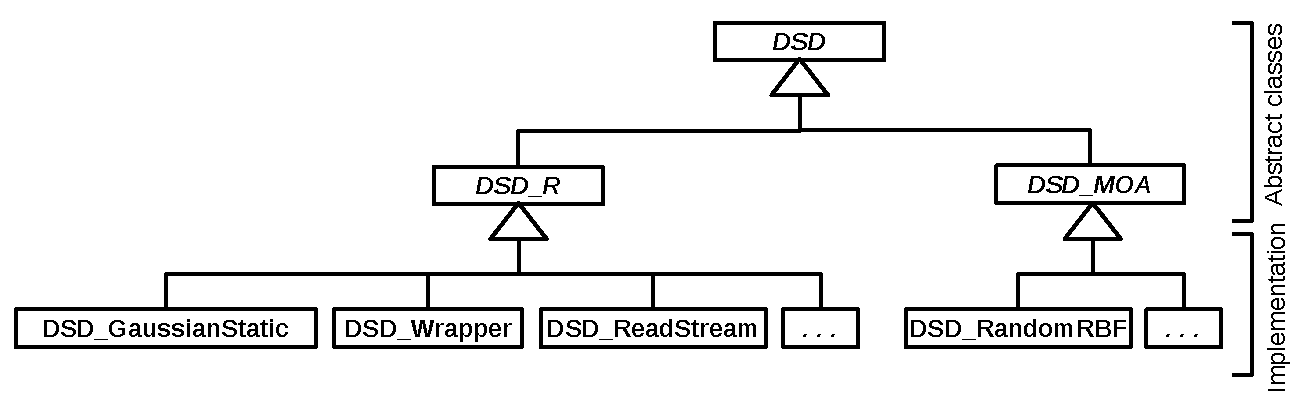
\includegraphics{dsd_uml}
\caption{UML diagram of the DSD architecture.}
\label{figure:dsd}
\end{figure}

The base class contains generic definitions for \code{get_points()} and \code{print()}, and each subclass contains a constructor function for specific object initialization. 


\hangpara{0.25in}{0}%
\code{get_points(x, n=1, ...)} – returns a matrix of data points from the DSD object \code{x}. The implementation varies depending on the class of \code{x}. The way this is done in \code{DSD_Gaussian_Static}, our general purpose DSD generator, is to first generate a vector of cluster numbers that determine which clusters the data points will be generated from. This vector is calculated according to the cluster probabilities given. Next, data points are iteratively generated up to \code{n} based on the \code{mu} and \code{sigma} for each cluster that was chosen from the data sampling. The size of each data point corresponds to the number of d dimensions initially defined during the creation of the DSD object.


\hangpara{0.25in}{0}%
\code{print()} – prints common attributes of the DSD object. Currently shown are the number of clusters, the number of dimensions, and a brief description of what implementation is generating the data points.


Unlike the MOA framework, the selected DSD holds no bearing on what DST is chosen; the two components act individually from one another (in MOA there are specific generators for classification and specific generators for clustering). It is up to the experimenter to choose the appropriate DSD for the behavior they are trying to simulate. Appendix A contains the user manual generated by \proglang{R} that discusses the exact details for each class implemented, and descriptions of the original algorithms they extend.


To accompany the assortment of DSD classes that read or generate data, we have also written a function called \code{write_stream()}. It allows the user to write \code{n} number of lines to an open \proglang{R} \code{connection}. Ideally it can be used in place of continually setting the seed of the random number generator when performing experiments. Instead, users will generate a set of data, write it to disk using \code{write_stream()}, read it back in using a \code{DSD_ReadStream}, and feed it to the DSTs being used in that particular experiment. We designed \code{write_stream()} so that the data points written to disk are written in chunks. Although this is slower than performing a single write operation to disk, this allows the user to theoretically write \code{n} points up to the limit of the physical memory of the system the software is running on.

\subsection{DataStreamTask}
\label{sec:design:dst}

After choosing a DSD class to use for data generation, the next step in the work flow is to define a DST. In \pkg{stream}, a DST refers to any data mining task that can be applied to data streams. We have purposefully left this ambiguous so that additional modules can be defined in the future to extend upon the DST base class. In general however, DSTs fall in two categories: data stream classification algorithms, and data stream clustering algorithms. In the current implementation of \pkg{stream} there are only \code{DataStreamClusterer} (DSC) classes define, but Figure~\ref{figure:dst} shows how additional tasks can easily extend from DST as shown by the addition of the abstract class \code{DataStreamClassifier} in the diagram. It is important to note that the concept of the DST class is merely for conceptual purposes--in the actual implementation of \pkg{stream} there is no direct implementation of DST because little is shared between the clustering and classification operations.


Extending from the base DST class are the class representations of two common data mining tasks: a DSC class for clustering, and a \code{DataStreamClassifier} class for classification. Under the DSC class, there is a further inheritance hierarchy in which \code{DSC_R} and \code{DSC_MOA} extend the base DSC class. This is to differentiate the underlying implementation details of each class under the two separate branches. Due to the state of our implementation, the following section will mainly focus on the DSC classes that have been developed, while also providing guidance on how the same principles can be applied to other data mining tasks such as classification.

\begin{figure}
\centering
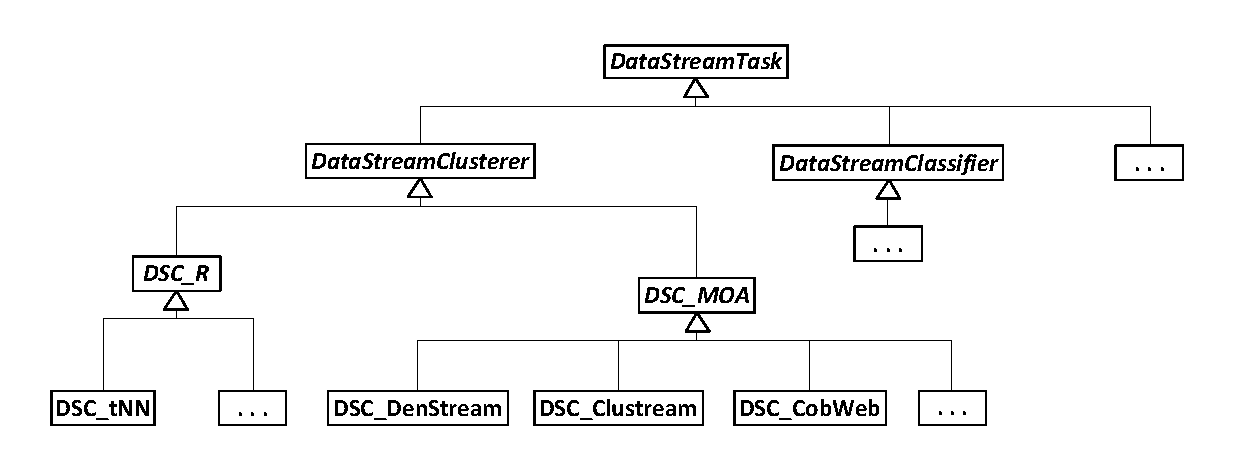
\includegraphics{dst_uml}
\caption{UML diagram of the DST architecture.}
\label{figure:dst}
\end{figure}

The base DSC class defines several functions that are inherited by each subclass. Similar to the architecture of the DSD class, each subclass must also provide a constructor individually.


\hangpara{0.25in}{0}%
\code{get_centers(x, ...)} – is a generic function that will return the centers--either the centroids or the medoids, depending on the algorithm--of the micro-clusters of the DSC object if any are available.


\hangpara{0.25in}{0}%
\code{nClusters(x)} – returns the number of micro-clusters in the DSC object if any are available.


\hangpara{0.25in}{0}%
\code{print(x, ...)} – prints common attributes of the DSC object. Currently it prints a small description of the underlying algorithm and the number of micro-clusters that have been calculated.


%%TODO: finish this explanation
\hangpara{0.25in}{0}%
\code{plot(x, ..., method="pairs")} – plots the centers of the micro-clusters. There are 3 available plot methods: pairs, plot, or pc. Pairs is the default method that does...

Currently the majority of the DSC classes that have been implemented use MOA implementations of the data stream clustering algorithm as their core and use lightweight \proglang{R} wrapper interfaces to communicate with the \proglang{Java} code. The only exception to this is \code{DSC_tNN} which is written entirely in \proglang{R} and uses some of \proglang{R}’s more advanced features to simulate mutable objects. Currently, the data stream clustering algorithms that are available in \pkg{stream} are StreamKM++ \citep{stream:Ackermann+Lammersen+Maertens+Raupach:2010}, threshold Nearest Neighbor as seen in \citep{stream:Hahsler+Dunham:2010, stream:Hahsler+Dunham:2010b}, ClusTree \citep{stream:Kranen+Assent+Baldauf+Seidl:2009}, DenStream \citep{stream:Cao+Ester+Qian+Zhou:2006}, Clustream \citep{stream:Aggarwal+Han+Wang+Yu:2003}, and CobWeb \citep{stream:Fisher:1987}.


It is important to note that many data stream clustering algorithms consist of two parts: an online component that clusters the incoming data points into micro-clusters, and an offline component that performs a traditional clustering algorithm on the micro-clusters. Our DSC implementations only include the online segment of these algorithms. This is to allow the user to choose how they would like to manipulate the micro-clusters during the offline face. For example, a user may want to only use a single DSC class, but may be interested in how different traditional clustering algorithms perform on the micro-clusters generated. As mentioned before, Appendix A contains all of the details concerning each implemented class.


\subsection{Class Interaction}
\label{sec:design:interaction}

Due to the abstraction in our workflow, the two step process will be similar for each combination of selected classes. Theoretically every DSD class will work flawlessly with any chosen DST class, although the results generated may not be optimal for every combination. Each subclass of the base DST also requires a set of input functions that will pull data from the DSD object and pass it to the DST object. In a classification example, these functions may be called \code{learn()} and \code{classify()} to signify the two main steps in data stream classification. For our implementation of the clustering task, we use a single function called \code{cluster()} to drive the interaction.


\hangpara{0.25in}{0}%
\code{cluster(dsc, dsd, n=1000)} – accepts  DSC object, a DSD object, and the number of points that will be generated by the DSD and passed to the DSC. Internally, \code{cluster()} also includes polymorphic implementations for each subclass of DSC, in this case, \code{DSC_R} and \code{DSC_MOA}. These internal implementations handle the different expectations by each DSC subclass: the MOA classes expect their data points to be packaged as Java Instance objects, while the R classes require no such packaging. It is important to note that underlying clustering within the DSC changes due to this process—no new clustering is created for each call to \code{cluster()}.


Figure~\ref{figure:interaction} demonstrates the interaction between a DSD object, a DSC object, and \code{cluster()}. After the clustering operation is finished, the results can be obtained from the DSC object by calling \code{get_centers()}, or they can be plotted directly to a chart by calling \code{plot()}.

\begin{figure}
\centering
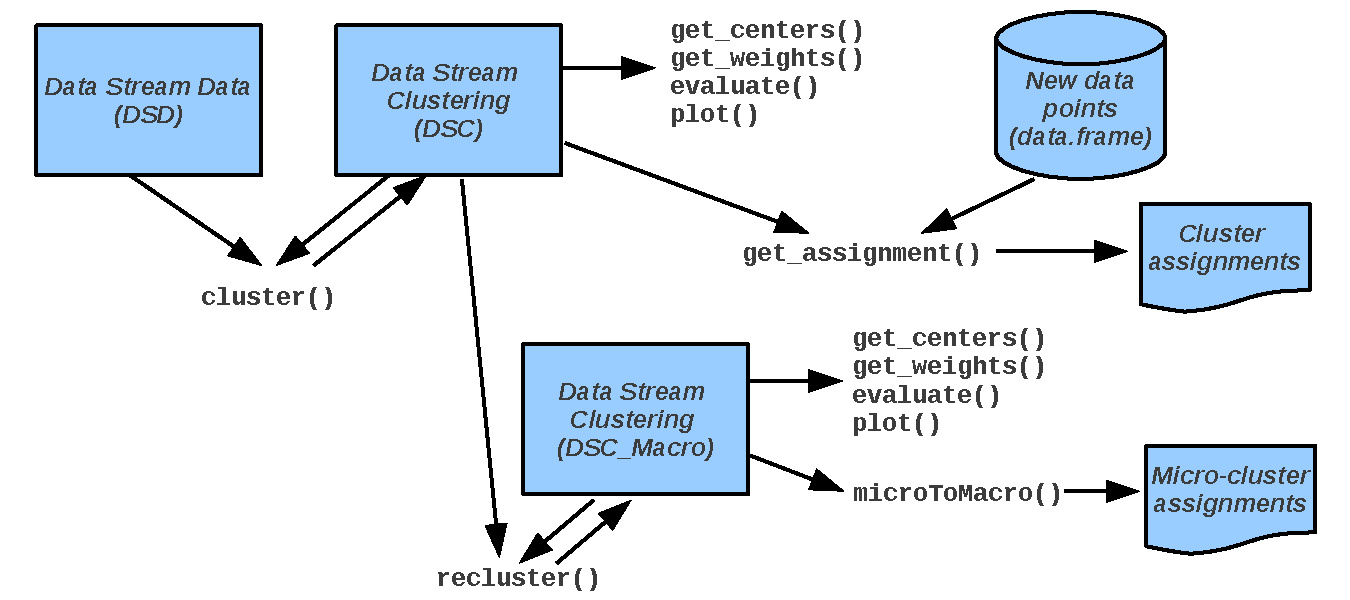
\includegraphics{interaction}
\caption{Interaction between the DSD and DSC classes}
\label{figure:interaction}
\end{figure}

\subsection{Extension}
\label{sec:design:extension}

In order to make our framework easily extendable, we developed a set of core functions that are necessary for each. As mentioned earlier, the actual \pkg{stream} implementation contains no definition for the DST concept--it is used only in the description of the design to show that all data stream mining tasks extend from the same base class. This section will outline the key functionality that needs to be available in the extension of the \pkg{stream} components. The core implementation of extension classes can be written in either \proglang{R}, \proglang{Java}, or \proglang{C}/\proglang{C++}, however, every class needs an \proglang{R} wrapper that can communicate with the rest of the framework.


DSD classes need a way to uniquely either generate or retrieve data that can be used as a stream for input to DST objects. Ideally, users will be able to alter the properties in the DSD class by passing parameters in the constructor. Common properties include the number of clusters to generate, the dimensionality of the data, the distribution of the data generated, how the data evolves over time, etc. Although these properties are desirable to control, it isn't always possible to do this in the implementation (similar to how we limit the input parameters of \code{DSD_MOA}). 


For DSD classes, there is only a single function in addition to a constructor that is needed in order to fulfill the interface, and that function is \code{get_points()}. This function simply returns an \proglang{R} matrix of the data created by the DSD. It is used mainly in the \code{cluster()} function to input data into DST objects that will perform data mining operations on them.

%%TODO: finish this section

Because the DST base class is The DST interface is a little more complicated in that there are currently 2 abstract classes that extend from the abstract base class, \code{DataStreamClusterer}.

\section{Examples}
\label{sec:examples}

Experimental comparison of data streams and algorithms is the main purpose of \pkg{stream}. In this section we give several examples in \proglang{R} that exhibit \pkg{stream}'s benchmarking capabilities. The examples become increasingly complex through the section. First, we start by giving brief introduction to the syntax of \pkg{stream} by using a pair of DSC and DSD objects. The second example shows how to save stream data to disk for use in later experiments. Finally, the last example demonstrates a detailed comparison of two algorithms from start to finish by first running the online component of two algorithms on the same data stream, then using \textit{k-means} to cluster the micro-clusters generated by each algorithm.

\subsection{Creating a data stream}
\label{examples:ds}

The first step in every example is to load the package.

\begin{Schunk}
\begin{Sinput}
> library("stream")
\end{Sinput}
\end{Schunk}

In this example, we would like to focus on the merits of the DSD class to model data streams. Currently there are 4 available classes: \code{DSD_Gaussian_Static}, \code{DSD_Gaussian_Dynamic}, \code{DSD_MOA}, and \code{DSD_ReadStream}. The syntax of creating an instance of each of the classes is consistent throughout. Below we show the creation of a \code{DSD_Gaussian_Static} object. We would like the data to be two dimensional, and to be generated by three clusters--these properties are shown as parameters during the instantiation. Because we have only defined two of the parameters, \code{mu}, \code{sigma}, \code{p}, and \code{noise} will be left to their default values. The \code{print()} function can display a brief summary of the DSD object.

\begin{Schunk}
\begin{Sinput}
> dsd <- DSD_Gaussian_Static(k = 3, d = 2)
> print(dsd)
\end{Sinput}
\begin{Soutput}
DSD - Data Stream Datasource: Static R Data Stream 
Number of clusters: 3 
Number of dimensions: 2 
\end{Soutput}
\end{Schunk}

Now that we have a DSD object created we can call functions on it to generate stream data. The most common of these functions is \code{get_points()}. It accepts a DSD object and a value \code{n} number of points and returns a numeric matrix composed of \code{n} rows and \code{d} columns. The points in this matrix are generated by different clusters defined during the creation of the DSD object. Additionally, we can set the parameter \code{assignment} in the \code{get_points()} function to \code{TRUE} to return vector that shows exactly which clusters the data points belong to. The \code{assignment} vector is shown in the code following.

\begin{Schunk}
\begin{Sinput}
> data <- get_points(dsd, 25, assignment = TRUE)
> data[, ]
\end{Sinput}
\begin{Soutput}
           [,1]      [,2]
 [1,] 0.9354351 0.9452162
 [2,] 0.9555359 0.8872530
 [3,] 0.3269630 0.9956624
 [4,] 0.9845553 0.8126872
 [5,] 0.9670650 0.9126810
 [6,] 0.8813410 0.6969180
 [7,] 0.4921329 1.0381927
 [8,] 0.8922827 0.8087074
 [9,] 0.9181655 0.7546756
[10,] 0.4104422 1.0034516
[11,] 0.9706034 0.8979045
[12,] 0.9330468 0.9621730
[13,] 0.9656003 0.7400985
[14,] 0.9903852 0.6330602
[15,] 0.3202613 0.9056487
[16,] 0.9661729 0.9783573
[17,] 0.2454538 0.8308899
[18,] 0.8445643 0.7365700
[19,] 0.3972626 1.0360031
[20,] 0.9721153 1.1037185
[21,] 0.7672246 0.6577269
[22,] 0.7531990 0.6743980
[23,] 0.8671167 0.6955512
[24,] 0.4795891 1.0944839
[25,] 0.9404588 1.1303063
\end{Soutput}
\begin{Sinput}
> attr(data, "assignment")
\end{Sinput}
\begin{Soutput}
 [1] 3 3 1 2 3 2 1 2 2 1 3 3 2 2 1 2 1 2 1 3 2 2 2 1 3
\end{Soutput}
\end{Schunk}

\code{n} can be of any size as long as the created matrix is able to fit into memory. The data produced can then be used in any choice of application. Because the data is two dimensional, we are able to easily plot it and identify which of the three clusters each data point comes from. Figure~\ref{figure:plot1} shows 1000 data points from the same DSD object with the identifiable clusters.

\begin{Schunk}
\begin{Sinput}
> plot(get_points(dsd, 1000))
\end{Sinput}
\end{Schunk}

\begin{figure}
\centering
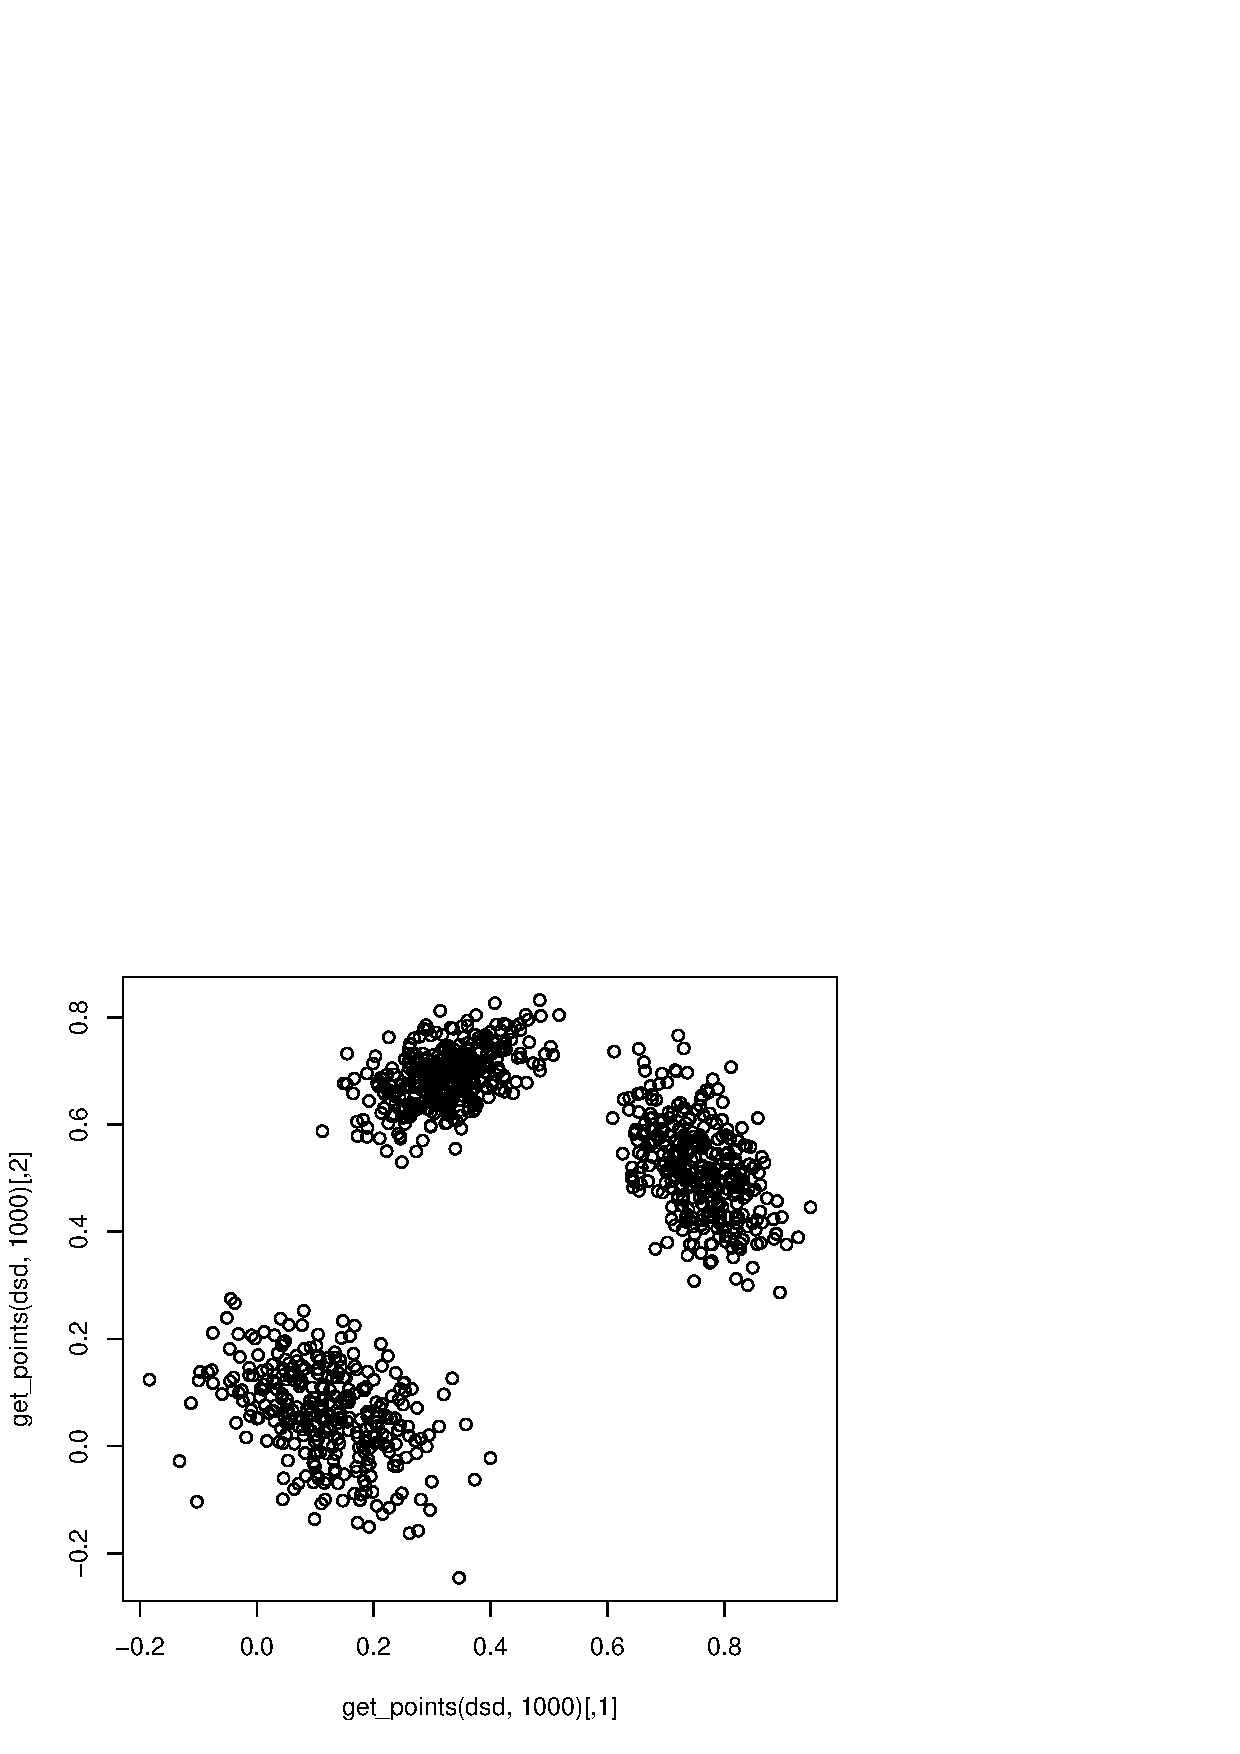
\includegraphics[width=.5\linewidth]{stream-plot1}
\caption{Plotting 100 data points from the data stream}
\label{figure:plot1}
\end{figure}

\subsection{Reading \& writing data streams to disk}
\label{examples:disk}

Sometimes it is nice to be able to access the data generated by the data streams outside of the \proglang{R} environment. \pkg{stream} has support for reading and writing data streams through an \proglang{R} \code{connection}. \code{connection}s can be opened to a number of different sources (see the \proglang{R} Reference Manual for a detailed explanation \citep{stream:R:2005}). In our example, we will focus on reading and writing to a file on disk.

We start by loading the package and creating a DSD object. In our DSD object we are using data with a dimensionality of 5 to demonstrate how large streams are stored on disk.

\begin{Schunk}
\begin{Sinput}
> library("stream")
> dsd <- DSD_Gaussian_Static(k = 3, d = 5)
\end{Sinput}
\end{Schunk}

Next, we write 100 data points to disk. The only constraint on the number of points written to disk is the physical constraint of hard disk space--only one data point is written at a time. While this may take slightly longer, we opted to take this route so that users would be able to write large amounts of data to disk in a single function call.

\code{write_stream()} accepts either a \code{connection} directly, or the file name to be written to. The \code{sep} parameter defines how the dimensions in each data point are separated. Behind the scenes we are using the \code{write.table()} function to write the data to disk. We are able to pass additional parameters to this function to alter how the data is written. In the code below we set the \code{col.names} parameter to \code{FALSE} so that the column names aren't also written to disk.

\begin{Schunk}
\begin{Sinput}
> write_stream(dsd, "dsd_data.txt", n = 100, sep = ",", col.names = FALSE)
\end{Sinput}
\end{Schunk}

This will create the file dsd\_data.txt (or overwrite it if it already exists) in the current folder and fill it with 100 data points from \code{dsd}. Now that the data is on disk, we can use a \code{DSD_ReadStream} object to open a connection to the file where it was written and treat it as a stream of data. \code{DSD_ReadStream} works in a way similar to \code{write_stream()} in that it reads a single data point in a time. Again, this allows us to read from files that may be several Gb without having to load all of the file into memory.

\begin{Schunk}
\begin{Sinput}
> dsd2 <- DSD_ReadStream("dsd_data.txt", sep = ",")
\end{Sinput}
\end{Schunk}

It is important that the \code{sep} parameter matches exactly the \code{sep} parameter used to write the stream to disk (the defaults are the same in the case that one wasn't defined explicitly). \code{DSD_ReadStream} objects are just like any other DSD object in that you can call \code{get_points()} to retrieve data points from the data stream. During the creation of a \code{DSD_ReadStream} object, there is an additional parameter, \code{loop}, that will discussed in the next example that allows us to replay the stream when the all of the data points from a connection have been read. 

\subsection{Replaying a data stream}
\label{examples:replay}

An important feature of \pkg{stream} is the ability to replay stream data. This ensures that all of the algorithms being experimented on will have the same data set and there won't be any anomalies due to concept drift in the data. We start this example is a similar manner, by loading the package and creating a DSD object. There are several ways to replay streams--one of them being to use a combination of \code{write_stream()} and \code{DSD_ReadStream} objects as mentioned in the previous example--but in this example we will discuss the use of the \code{DSD_DataFrame} class.

The \code{DSD_DataFrame} class was designed with the intent of being a wrapper class for data that has already been generated in the form of a data frame or matrix. Because of this feature, we are able to use data produced from another data stream and wrap it in a \code{DSD_DataFrame} object to replay the data. Similar to the \code{DSD_ReadStream} class, there is also a \code{loop} parameter in \code{DSD_DataFrame}. The \code{loop} parameter, when set to \code{TRUE}, will loop over the data points within the data stream when all of them have been used. For instance, if there are 10 data points in the object, and the user requests 100 in a call to \code{get_points()}, with looping enabled the 10 data points will be returned 10 times to give the user the request 100 data points. In our example we opt to leave the \code{loop} parameter as its default, \code{FALSE}.

\begin{Schunk}
\begin{Sinput}
> library("stream")
> dsd <- DSD_Gaussian_Static(k = 3, d = 2)
> replayer <- DSD_DataFrame(get_points(dsd, 100), k = 3)
\end{Sinput}
\end{Schunk}

Just like the \code{DSD_ReadStream} object created in the previous example, the \code{replayer} variable can be used like any other DSD object. When all of the data points have been used in the stream, there is a function available called \code{reset()} which returns the \code{DSD_DataFrame} to its original state (\code{reset()} is also available for \code{DSD_ReadStream} objects. 

\begin{Schunk}
\begin{Sinput}
> dsc <- DSC_Clustream()
> cluster(dsc, replayer, 100)
> reset_stream(replayer)
\end{Sinput}
\end{Schunk}

\subsection{Clustering a data stream}
\label{examples:clustering_ds}

Again, start by loading \pkg{stream}.

\begin{Schunk}
\begin{Sinput}
> library("stream")
\end{Sinput}
\end{Schunk}

Next, create the DSC and DSD objects. In this example we use the \code{DSC_DenStream} with its default parameters, and \code{DSD_MOA} with 2 dimensionality data generated from 3 clusters.

\begin{Schunk}
\begin{Sinput}
> dsc <- DSC_DenStream()
> dsd <- DSD_MOA(k = 3, d = 2)
\end{Sinput}
\end{Schunk}

Now, the objects need to interact with one another through the \code{cluster()} function. The clustering operation will implicitly alter \code{dsc} so no reassignment is necessary. By default, \code{DSC_DenStream} is initialized with 1000 points, meaning that no new micro-clusters are created until this threshold has been breached, which is why we cluster 2000 new data points.

\begin{Schunk}
\begin{Sinput}
> cluster(dsc, dsd, 2000)
\end{Sinput}
\end{Schunk}

After clustering the new data, we are ready to view the results. It is important to note that we have to call \code{get_points()} on \code{dsd} again to obtain new data points to plot against. These are not the same data points used in the initial clustering, so the micro-clusters may not fit exactly, but because they are randomly generated it should be an accurate fit.

\begin{Schunk}
\begin{Sinput}
> plot(dsc, col = "red", pch = 3)
> points(get_points(dsd, 1000), col = "grey")
\end{Sinput}
\end{Schunk}

\begin{figure}
\centering
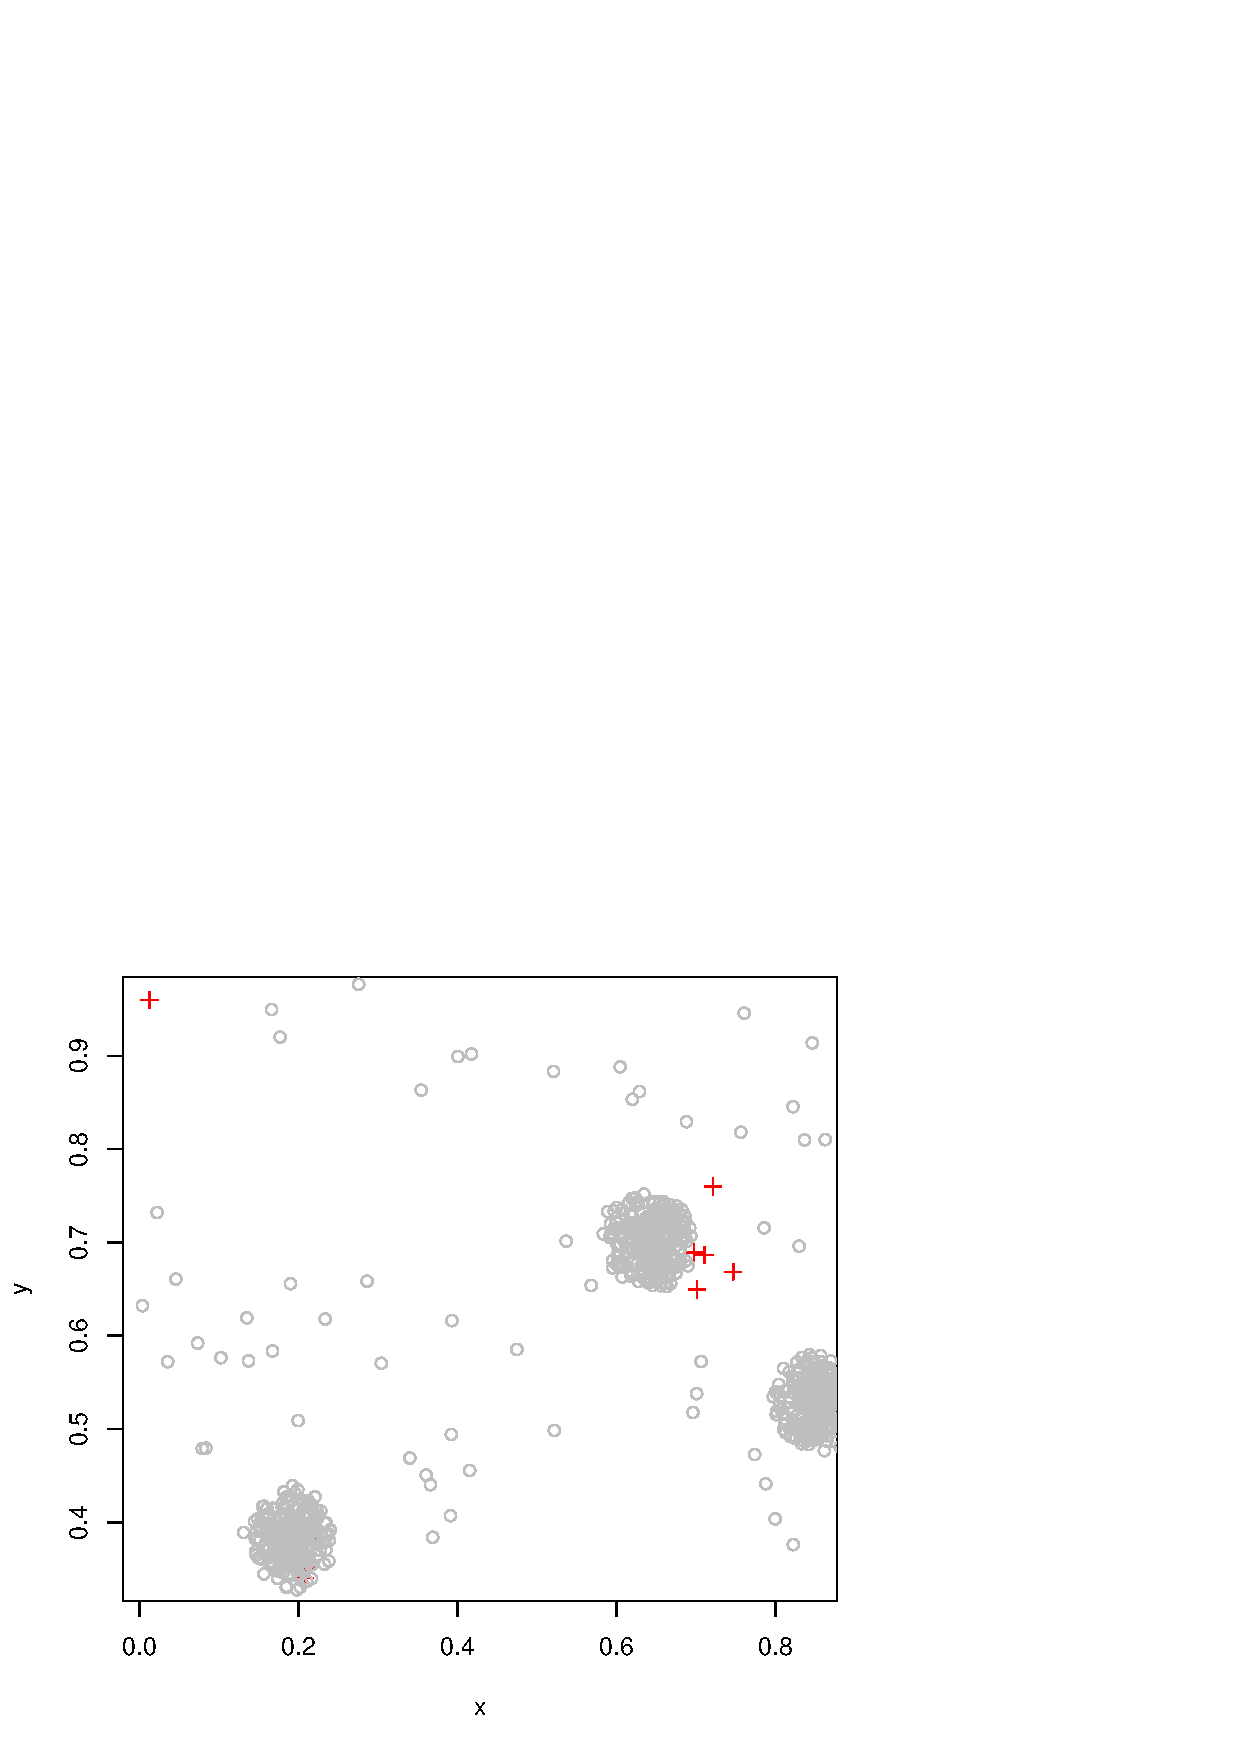
\includegraphics[width=.5\linewidth]{stream-plot2}
\caption{Plotting the micro-clusters on top of data points}
\label{figure:plot2}
\end{figure}

Figure~\ref{figure:plot2} is the result of the calls to \code{plot()} and \code{points()}. It shows the micro-clusters as red crosses on top of grey data points. It is often helpful to visualize the results of the clustering operation during the comparison of algorithms.

\subsection{Full experimental comparison}
\label{examples:full}

This example shows the \pkg{stream} framework being used from start to finish. It encompasses the creation of data streams, clusterers, the online clustering of data points as micro-clusters, and then the comparison of the offline clustering of 2 data stream clustering algorithms by applying the \textit{k-means} algorithm. As such, less detail will be given in the topics already covered in the previous examples and more detail will be given on the comparison of the 2 data stream clustering algorithms.

\begin{Schunk}
\begin{Sinput}
> # setting up the experiment
> library("stream")
> dsd <- DSD_DataFrame(get_points(DSD_Gaussian_Static(k=3, d=2), 10000), k=3)
> dsc1 <- DSC_DenStream(initPoints=50)
> #dsc2 <- DSC_Clustream()
> 
> # clustering the data
> cluster(dsc1, dsd, 100)
> reset_stream(dsd)
> #cluster(dsc2, dsd, 100)
> #reset_stream(dsd)
> 
> # plotting the data, and the 2 sets of micro-clusters generated
> d <- get_points(dsd, 100)
> plot(d, xlab='x', ylab='y', pch=4, cex=.5)
> points(get_centers(dsc1),col='red', cex=2,lwd=2)
> #points(get_centers(dsc2),col='blue', cex=2,lwd=2)
\end{Sinput}
\end{Schunk}

\begin{figure}
\centering
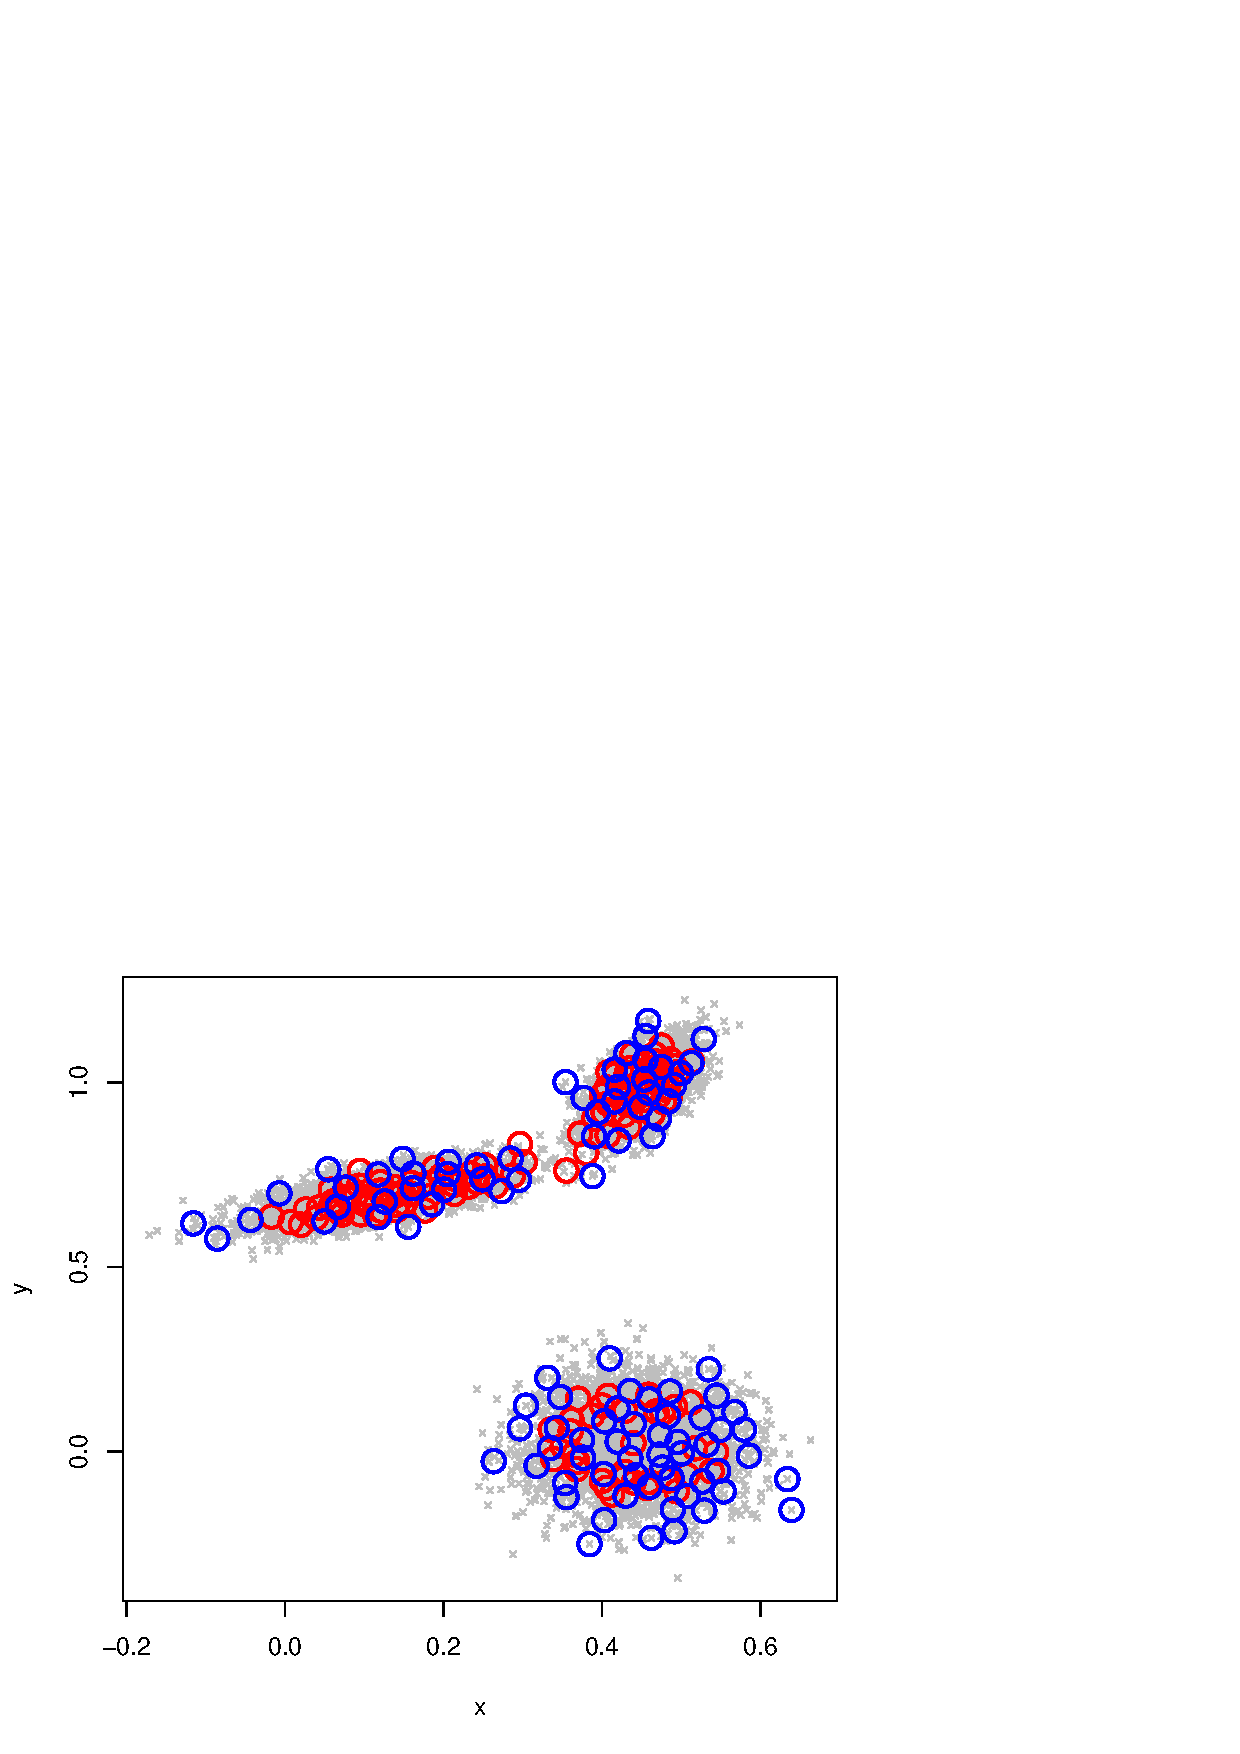
\includegraphics[width=.5\linewidth]{stream-plot3}
\caption{Plotting 2 sets of different micro-clusters against the generated data}
\label{figure:plot3}
\end{figure}

The code above creates a \code{DSD_DataFrame} object from a \code{DSD_Gaussian_Static} object so that we can replay the same stream data for both DSC objects. We then use the \code{DSD_DataFrame} to feed the exact data stream into 2 different algorithms, DenStream and Clustream, during the \code{cluster()} operation. Note that after each call to \code{cluster()}, we also have to call \code{reset_stream()} to reset the \code{DSD_DataFrame} back to its original position.


After the clustering operations, we plot the calculated micro-clusters and the original data. Figure~\ref{figure:plot3} shows the 2 sets of micro-clusters created, in red and blue, over the original data which is in black. We have plotted the micro-clusters as circles to more closely reflect their nature, however, the circles are merely a representation and the radii haven't been calculated specifically for each micro-cluster. The plot makes it easy to point out differences in the two algorithms. The DenStream micro-clusters, in red, stay true to the nature of the algorithm in that they congregate where their is a large number of data points; there clustering of these micro-clusters in these dense areas. Clustream on the other hand, in blue, is more evenly spread, and the micro-clusters are relatively separated, covering most of the area that the generated data fills.


We can then take this a step further. Figure~\ref{figure:plot4} shows a new plot--in this case, we are plotting the calculated "macro" clusters of each algorithm as a result of a \textit{k-means} operation. We use the term "macro" here to differentiate the clusters from \textit{k-means} from the micro-clusters generated by the stream clustering algorithms. Again, the DenStream clusters are shown in red, and the Clustream clusters are shown in blue. We have enlarged the circle representations for the \textit{k-means} clusters to better show the area they cover.

%%TODO: how do we make this a continuation of the previous chunk without having to re-enter all the commands??
\begin{Schunk}
\begin{Sinput}
> plot(d, xlab = "x", ylab = "y", pch = 4, cex = 0.5)
> points(kmeans(get_centers(dsc1), 3)$centers, col = "red", cex = 10, 
+     lwd = 2)
\end{Sinput}
\end{Schunk}

This last operation is an example of how we use the same offline component for two different algorithms, and the differences that it produces. \proglang{R} contains an assortment of traditional clustering algorithms that are available through the installation of various packages. It is up to the user to decide which clustering algorithm they would like to use as the offline component. Most stream clustering algorithms are developed with a certain offline algorithm in mind, but it is interesting to see the different combinations of algorithms and the results they produce.


There are several external packages that are required to use the \pkg{stream} package. These include the \pkg{proxy} package, written by \cite{stream:Meyer+Buchta:2010}, the \pkg{MASS} package by \cite{stream:Venables+Ripley:2002}, and \pkg{clusterGeneration} by \cite{stream:Qiu+Joe:2009}. To facitilate the communication between \proglang{R} and \proglang{Java}, we used the \pkg{rJava} \citep{stream:Urbanek:2010}. This allowed us to make method calls directly to the JRI from within the \proglang{R} environment. The \pkg{stream} Reference Manual is available in the appendix. It documents all of the available classes and functions, as well as the details behind their implementation.

\begin{figure}
\centering
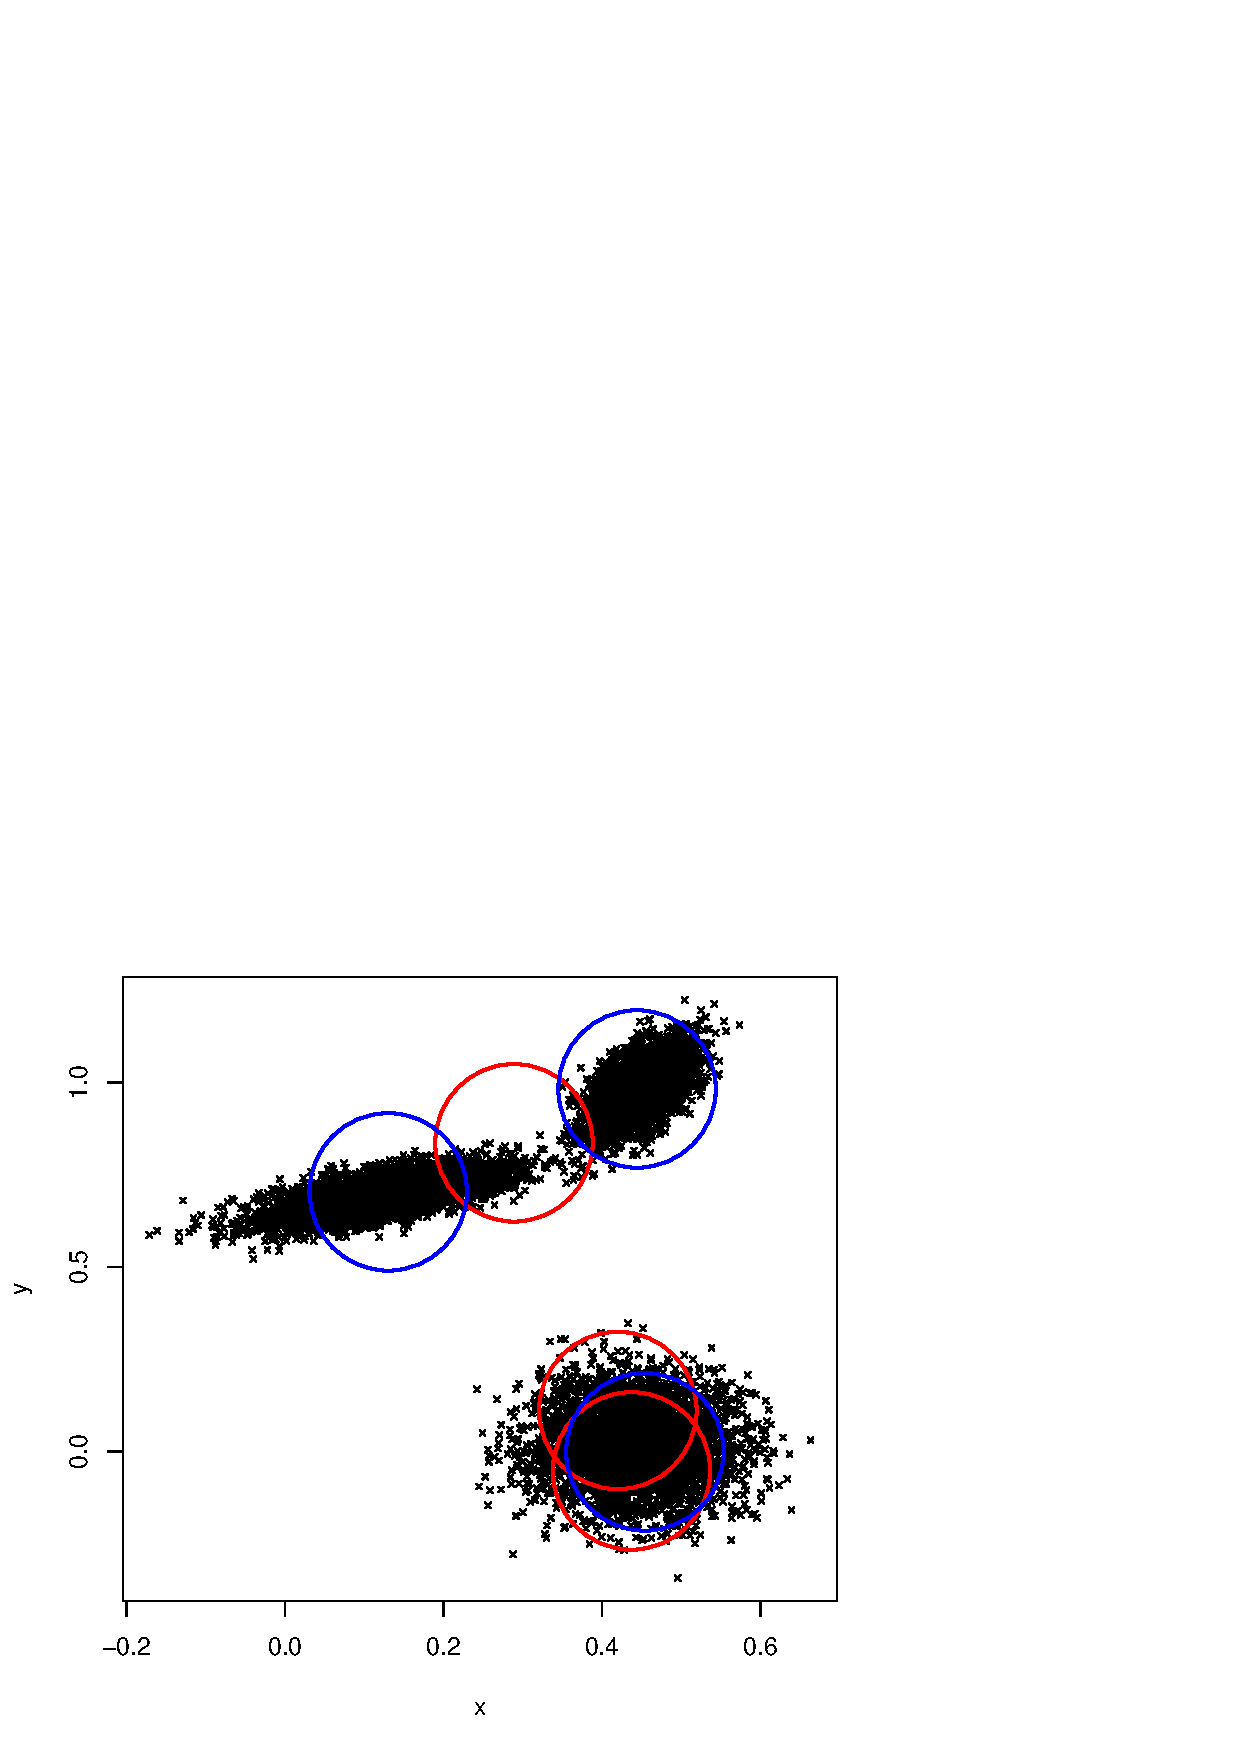
\includegraphics[width=.5\linewidth]{stream-plot4}
\caption{Plotting the results of a \texit{k-means} operation on each stream clustering algorithm}
\label{figure:plot4}
\end{figure}

\section{Conclusion \& Future Work}
\label{sec:conclusion}

\pkg{stream} is a data stream modeling framework in \proglang{R} that has both a variety of data stream generation tools as well as a component for performing data stream mining tasks. The flexibility offered by our framework allows the user to create a multitude of easily reproducible experiments to compare the performance of these tasks.


Furthermore, the infrastructure that we have built can be extended upon in multiple locations. We have abstracted each component to only require a small set of functions that are defined in each base class. Writing the framework in \proglang{R} means that developers have the ability to design components either directly in \proglang{R}, or design components in \proglang{C}/\proglang{C++} or \proglang{Java}, and then write an \proglang{R} wrapper to use the high level code. Upon completion, stream will be available from the R-Forge website for download.


In the future, we plan on adding additional functionality to \pkg{stream}. Currently we only have implementations for clustering tasks; we would like to develop a classification module that also extends from the base DST class. Additionally, there are plans to develop an evaluation module that accompanies each DST class to provide immediate feedback on their. Finally, for each of the DST classes developed, we would like to include all of the available algorithms, both the latest innovations and the original algorithms that shaped the research for the respective area.


\bibliography{stream}

%%\appendix
%%\section{stream Reference Manual}
%%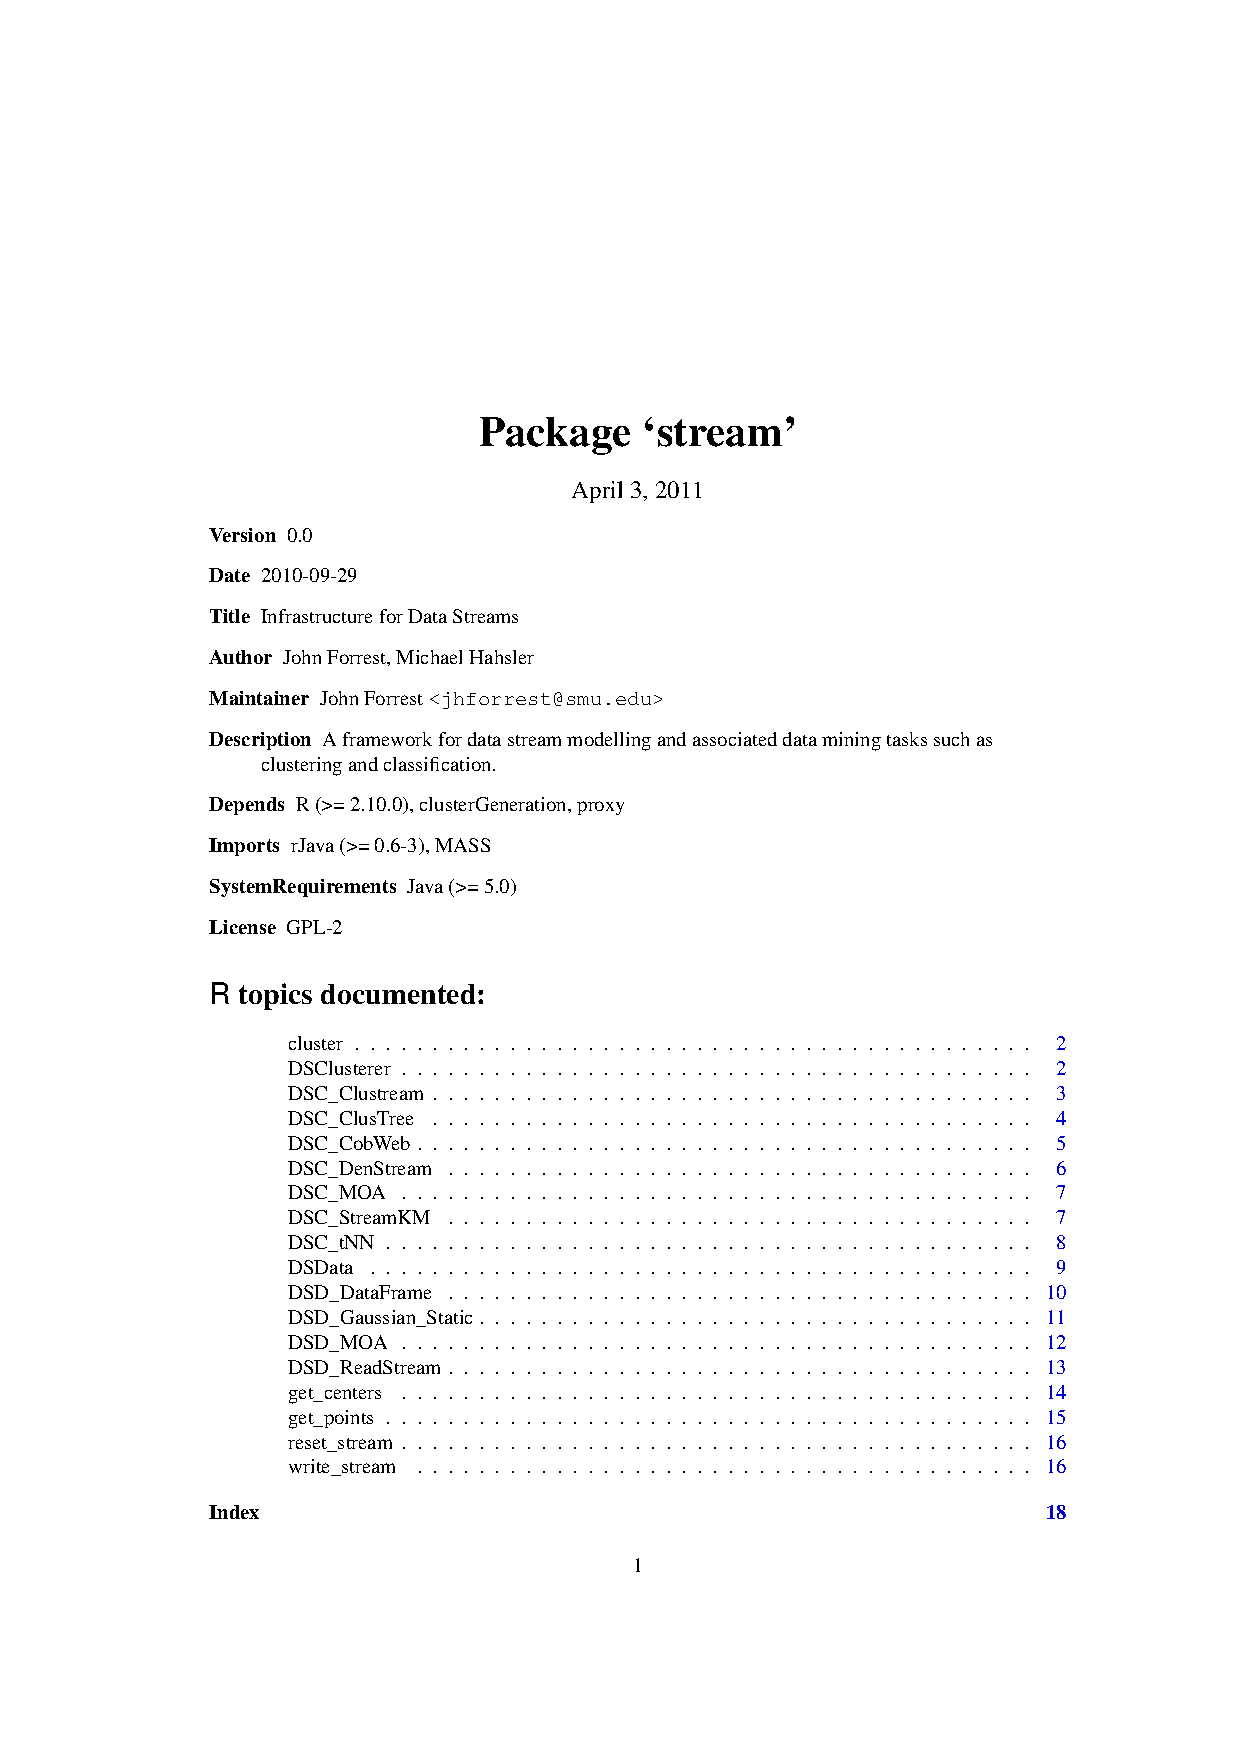
\includepdf[pages=-]{manual.pdf}

\end{document}
